\documentclass[12pt]{article}
\usepackage{latexsym}
\usepackage{amssymb,amsmath}
\usepackage[pdftex]{graphicx}
\usepackage{listings}
\usepackage{color}

\definecolor{dkgreen}{rgb}{0,0.6,0}
\definecolor{gray}{rgb}{0.5,0.5,0.5}
\definecolor{mauve}{rgb}{0.58,0,0.82}

\lstset{frame=tb,
  language=Java,
  aboveskip=3mm,
  belowskip=3mm,
  showstringspaces=false,
  columns=flexible,
  basicstyle={\small\ttfamily},
  numbers=none,
  numberstyle=\tiny\color{gray},
  keywordstyle=\color{blue},
  commentstyle=\color{dkgreen},
  stringstyle=\color{mauve},
  breaklines=true,
  breakatwhitespace=true,
  tabsize=3
}

\topmargin = 0.1in \textwidth=5.7in \textheight=8.6in

\oddsidemargin = 0.2in \evensidemargin = 0.2in


\begin{document}

\title{Experimentation with Clustering Algorithms}

\author{Corinne Curcie and Shivam Naik}
\date{March 5, 2017}

\maketitle

\begin{abstract}
Clustering algorithms are a popular tool for making sense of big data. Our project involved implementing various algorithms, focusing specifcally on high-dimensional data, to gain better understanding . 
\end{abstract}


\begin{enumerate}

\item Introduction

\item Related Work

\item Algorithms Implemented

\textbf{3.1 K-Means}

One of the algorithms we implemented is a variant on K-Means. Before getting into the details of that algorithm, we will go over the basics of K-Means, since we also used it as a benchmark when scoring preformances of algorithms we implemented. The well-known K-Means algorithm starts by choosing $k$ points in the dataset to be the initial cluster center points, and then updates on an ``expectation-maximization mechanism'' (EM).\\
 The ``E-step'' is the cluster assignment step, where points are labelled with a cluster based on which of the center points they are closest to. The ``M-step'' is the update step, where the $k$ cluster center points are recalculated to be some average of all of the points that were labeled as belonging to that cluster during the previous ``E-step'' round. The algorithm stops when the change in centers from one round to the next is less than some predetermined threshold. The objective function that K-Means tries to minimize is the sum of squared Euclidean distances from each point to its assigned cluster center:

$$ {\underset {\mathbf {S} }{\operatorname {arg\,min} }}\sum _{i=1}^{k}\sum _{\mathbf {x} \in S_{i}}\left\|\mathbf {x} -{\boldsymbol {\mu }}_{i}\right\|^{2} $$

\textbf{3.2 K-Subspaces}

We were intrigued by a 2009 paper that proposed a ``K-Subspaces" algorithm similar to K-Means (Wang, Ding, and Li 2009). Instead of using Euclidean distances for our objective function, multiple distance measures are used during the ``E-step'' to determine which centers the points are closest to. The authors of the algorithm decided to focus on three possible subspaces -- 1D lines, 2D planes, and 3D spheres -- and determines distance functions based on those subspaces. By calculating all three distances for each pair of point and cluster center, the algorithm is better able to determine when a point is within a cluster of a non-standard space. To extend this performance not only to the entire dataset but also subspaces within the dataset, PCA is used during distance calculations to isolate meaningful subspaces

\textbf{K-Subspaces Initialization} 

For initializing cluster centers before beginning the EM steps, we used the standard ``K-means++'' algorithm, which probabilistically selects initial clusters. Specifically, the algorithm goes through the following steps: (1) Select an input data point uniformly at random to be the first center. (2) Calculate the distance between every point $x$ and its nearest center point that has already been chosen. (3) Select a new data point as a next center, using a probability distribution where a point is chosen with probability proportional to the distance calculated in step 2. (4) Repeat the steps 2 and 3 until $k$ centers have been chosen. The ``K-means++'' initialization is also used in scikit-learn’s implementation of K-Means.

\textbf{Cluster Assignment Step}

In our cluster assignment step is when we use the new distance measures proposed by the authors. Instead of finding the direct distance to the center of a cluster, they aim to estimate a $\textit{surface}$ of a cluster by using perpendicular distances. For the following equations, let $x$ be a point and $C_k$ represent a cluster where $c_k$ is the center point of the cluster. 

\smallskip
\textbf{Line Distance:}

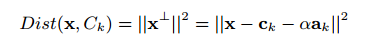
\includegraphics[scale=0.75]{eq1.png}

where

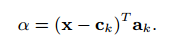
\includegraphics[scale=0.75]{eq12.png}

Here, $a_k$ represents the first principal component vector found using PCA.

\textbf{Plane Distance:}

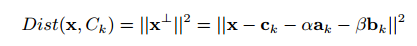
\includegraphics[scale=0.75]{eq2.png}

where 

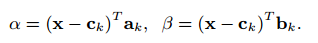
\includegraphics[scale=0.75]{eq22.png}

Here, $a_k$ again represents the first principal component vector found using PCA, and $b_k$ is the second principal component.

\smallskip

\textbf{Sphere Distance:}

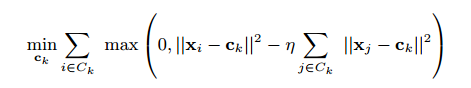
\includegraphics[scale=0.75]{eq3.png}




\item Datasets Used

\item Performance

\textbf{K-Subspaces on Synthetic Data}

 For our synthetic data, we wanted to demonstrate the ability to cluster for a variety of shapes. Data includes 1D lines, 2D planes, and 3D spheres, and the goal is for K-subspaces to cluster those shapes together separately even when they are close together. 



\end{enumerate}

\end{document} 
